\chapter{Local Flatness, Covariant Derivatives, and Curvature}

General relativity has the reputation of being conceptually forbidding, but this lecture begins by cutting that impression down to size. The ideas are not the impossible part. The nuisance is the notation, the index bookkeeping, and the sheer amount of calculation that the subject demands. It is therefore sensible to proceed patiently and concretely. These companion notes follow Leonard Susskind's lecture in that spirit; where the blackboard itself carries mathematical weight, we retain supporting board evidence from the archival work of LazyingArt LLC and Video2Book.

\section{Why We Need a Diagnostic for Curvature}

Susskind begins by conceding the obvious: general relativity is hard to calculate with. One can compress the notation, and experts often do, but for a first serious pass it is better to see the indices rather than hide them. The lecture then makes a brief detour through modern research, only to come back to the real point: this is the last lecture on Riemannian geometry by itself. The next step will be gravity, and the bridge to gravity is a sharply formulated geometric question.

The question is this. Suppose we are handed a metric \(g_{mn}(x)\). How do we tell whether there is genuine curvature, or whether we are merely using awkward coordinates? This is exactly the same mathematical problem as distinguishing a real gravitational field from a mere coordinate effect.

There is an obviously bad way to do it. We could search through all possible coordinate systems, transform the metric again and again, and ask whether in some lucky coordinate system it becomes the flat metric \(\delta_{mn}\). But this is hopeless. It is an infinite search.

The good way is to construct a diagnostic quantity out of the metric and its derivatives. Better still, it should be a tensor. If a tensor vanishes in one coordinate system, it vanishes in all coordinate systems. Thus we are looking for a tensorial object whose vanishing everywhere is equivalent to flatness. Susskind names the target early: it is the curvature tensor. The rest of the lecture is the machinery needed to earn that answer rather than merely announce it.

\section{Metric Review: The Minimum Needed Machinery}

Before reaching curvature, the lecture deliberately backs up. We start, simply, with a space. In one dimension there is almost no geometry beyond total length: a closed loop of rope can be bent and wiggled in many ways, but a bug walking on it can detect only the intrinsic length. In two dimensions the situation becomes richer. Planes, spheres, lumpy surfaces, and tori are intrinsically different, and what characterizes them is the metric tensor.

The metric tells us how to compute the squared length of an infinitesimal displacement:
\begin{equation}
ds^2 = g_{mn}\,dx^m dx^n.
\end{equation}
Because \(ds^2\) is an invariant, the object \(g_{mn}\) must transform as a tensor. That fact is not ornamental. It is the reason the metric can carry geometric content independent of the coordinates used to describe it.

The metric also has an inverse,
\begin{equation}
g^{mr}g_{rn}=\delta^m{}_n,
\end{equation}
and in Riemannian geometry it is positive definite. Equivalently, for every nonzero displacement \(u^m\),
\begin{equation}
g_{mn}u^m u^n>0.
\end{equation}
Susskind emphasizes that this is a specifically Riemannian statement. Later, when we move to Einsteinian geometry, the signature changes and this positivity property is lost.

The metric also lets us raise and lower indices. For the lecture, this is needed only at the basic level:
\begin{align}
V_n &= g_{nm}V^m,\\
V^m &= g^{mn}V_n.
\end{align}
These are not two different vectors. They are two coordinate descriptions of the same geometric object.

A useful preliminary observation now enters. If the components \(g_{mn}\) were constant in space, then by a suitable linear change of coordinates one could straighten the angles and bring the metric to \(\delta_{mn}\). In that case the space would certainly be flat. What makes the problem interesting is precisely the position dependence of the metric.

There is another point here that is worth stating carefully because Susskind insists on it later in the course: it is not correct to say that a flat space \emph{is} the metric \(\delta_{mn}\). What is correct is that in suitable coordinates a flat metric can be expressed by the components \(\delta_{mn}\). The distinction matters, because the same flat geometry may look nontrivial in curvilinear coordinates.

\section{Gaussian Normal Coordinates and Local Flatness}

At this stage the lecture asks a natural question: to what extent can an arbitrary metric be made to look flat by a clever choice of coordinates? The answer is local, and the local answer is powerful.

\begin{theorem}
At any point \(x_0\) of a smooth Riemannian space, one can choose Gaussian normal coordinates such that
\begin{align}
g_{mn}(x_0) &= \delta_{mn},\\
\partial_r g_{mn}(x_0) &= 0,
\end{align}
while in general the second derivatives cannot all be made to vanish:
\begin{equation}
\partial_r\partial_s g_{mn}(x_0)\neq 0
\qquad \text{in general.}
\end{equation}
\end{theorem}

\begin{figure}[h]
\centering

\includegraphics[width=0.82\textwidth]{lecture_03_figure_03.png}
\caption{Board statement of the Gaussian normal conditions for the metric.}
\end{figure}

The lecture presents these statements first geometrically. We go to a point, choose axes there, and extend them as straight as the geometry permits. Later this ``as straight as possible'' will become the language of geodesics. For the moment the point is simpler: there are coordinates, good in the immediate vicinity of the chosen point, in which the metric looks Euclidean and its first derivatives vanish.

\subsection{Question \& Answer}

\paragraph{Question.} Is this simplification only at one point, or does it extend through a region?

\paragraph{Answer.} Only at the chosen point. One may choose Gaussian normal coordinates at every point, but not one single coordinate system that achieves this throughout an extended region unless the space is actually flat. Away from the chosen point the second derivatives of the metric begin to show themselves, and that is precisely where the intrinsic geometry starts to reappear.

This is the first major lesson of the lecture. Flatness to zeroth and first order carries no invariant content. It can always be arranged. Whatever truly detects curvature must therefore live at second order.

Susskind then gives a counting argument. Take the point of interest to be the origin and suppose we begin with some coordinates \(y^m\). We look for new coordinates \(x^m\) having the same origin and expanded in powers of \(y\):
\begin{equation}
x^m = y^m + C^m{}_{nr}\,y^n y^r + O(y^3).
\end{equation}
The blackboard writes only the quadratic part explicitly,
\[
x^m = y^m + C^m{}_{nr}\,y^n y^r,
\]
and that is enough for the counting argument.

In four dimensions there are
\begin{equation}
\frac{4\cdot 5}{2}=10
\end{equation}
independent quadratic monomials \(y^n y^r\). For each choice of the upper index \(m\), this gives ten coefficients, so altogether there are
\begin{equation}
4\times 10 = 40
\end{equation}
adjustable quadratic coefficients.

On the other hand, the symmetric metric \(g_{mn}\) has ten independent components, and requiring that each of their four first derivatives vanish at the origin gives
\begin{equation}
10\times 4 = 40
\end{equation}
conditions. Forty unknown coefficients against forty first-derivative conditions: the balance is exactly right. This is why the first derivatives can be killed at a point.

But the counting does not continue indefinitely. At the next order one no longer has enough freedom to remove all higher derivatives. So the second derivatives survive in general, and those second derivatives are exactly what the curvature tensor will probe.

This is why every smooth metric is locally flat in the sense relevant to the lecture. It is not flat globally, and it is not necessarily flat even in a neighborhood beyond first order. But at one point, and through first derivatives, the geometry can always be made to imitate Euclid.

\section{Why Ordinary Derivatives of Vector Components Fail}

Gaussian normal coordinates are introduced for a reason. The next task is to define what it means to differentiate a tensor, and in particular a vector, in a way that is independent of coordinates.

The naive thought is irresistible. If a vector field has components \(V_m(x)\), why not simply differentiate the components? Why not say that \(\partial_r V_m\) is the derivative of the vector? The lecture now slows down and shows why that fails.

Imagine, first, a locally straight coordinate system: in flat space these would just be Cartesian coordinates, and in curved space they are Gaussian normal coordinates at the point of interest. Now superimpose on them another coordinate system whose coordinate lines curve from point to point. A vector that is geometrically ``the same'' at two neighboring points can nevertheless have different components in the curved coordinates, simply because the coordinate axes themselves have rotated or distorted.

\begin{figure}[h]
\centering

\includegraphics[width=0.9\textwidth]{lecture_03_figure_02.png}
\caption{Coordinate transformation, local geometric sketch, and the boxed naive condition that fails to be tensorial.}
\end{figure}

The boxed blackboard condition is therefore exhibited as a deliberate mistake:
\begin{equation}
\frac{\partial V_m}{\partial x^r}=0.
\end{equation}
The lecture's point is not that this equation is always false. The point is that it is not tensorial. It can be true in one coordinate system and false in another.

\subsection{Question \& Answer}

\paragraph{Question.} Why can all these derivatives vanish in one coordinate system but not in another?

\paragraph{Answer.} Because the change may be coming from the coordinates rather than from the vector. In a locally straight frame, a constant vector field really does have constant components. But in a curvilinear frame the basis directions themselves vary from point to point. The components then change even when the geometric vector does not. So the vanishing of \(\partial_r V_m\) is not an invariant statement.

This is the precise obstacle. If \(\partial_r V_m\) were the components of a rank-\((0,2)\) tensor, then once they vanished in one coordinate system they would vanish in all coordinate systems. Since that is not so, ordinary derivatives of vector components cannot themselves be tensor components.

\begin{figure}[h]
\centering
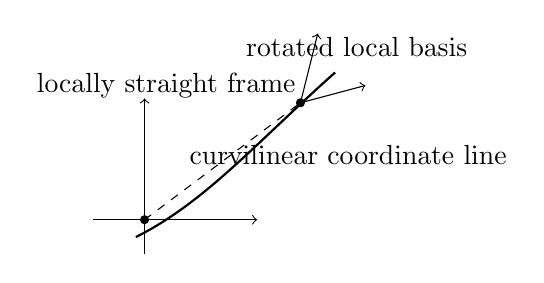
\begin{tikzpicture}[scale=1.1]
\draw[->] (-0.6,0) -- (1.3,0);
\draw[->] (0,-0.4) -- (0,1.4);
\fill (0,0) circle (1.5pt);
\draw[thick] (-0.1,-0.2) .. controls (0.7,0.2) and (1.3,0.9) .. (2.2,1.7);
\fill (1.8,1.35) circle (1.5pt);
\draw[->] (1.8,1.35) -- (2.55,1.55);
\draw[->] (1.8,1.35) -- (2.0,2.15);
\draw[dashed] (0,0) -- (1.8,1.35);
\node at (0.25,1.55) {locally straight frame};
\node at (2.35,0.75) {curvilinear coordinate line};
\node at (2.45,2.0) {rotated local basis};
\end{tikzpicture}
\caption{Schematic reconstruction of the lecture's local-frame comparison. The geometric vector may stay the same while the coordinate directions rotate from point to point.}
\end{figure}

So the lecture now has its first genuine tension: we need a derivative that agrees with ordinary differentiation in the best possible local coordinates, but remains a tensor after we return to arbitrary coordinates.

\section{Covariant Derivative and the Christoffel Symbols}

The covariant derivative is introduced operationally rather than axiomatically. To differentiate a vector at a point, we first build Gaussian normal coordinates near that point. In those coordinates the metric is as flat as possible and the coordinate directions vary as little as possible. We then compare neighboring vectors by shifting one back to the base point while keeping its Gaussian-normal components fixed. The ordinary derivative computed in those Gaussian normal coordinates is taken to define the true derivative.

Only after that do we transform back to arbitrary coordinates. When this is done, the answer is not just an ordinary partial derivative. There is an additional term that accounts for the fact that the coordinates themselves are changing from point to point. In normalized notation, for a covariant vector we write
\begin{equation}
\nabla_r V_m = \partial_r V_m - \Gamma^{t}{}_{rm}V_t.
\end{equation}
Here \(\nabla_r V_m\) is the covariant derivative, and \(\Gamma^{t}{}_{rm}\) is the connection coefficient, or Christoffel symbol.

In Gaussian normal coordinates at the chosen point, the extra term disappears:
\begin{equation}
\Gamma^{t}{}_{rm}(x_0)=0.
\end{equation}
That is exactly why the construction starts there. We differentiate in the coordinate system closest to Cartesian coordinates, and only then transform back.

The same pattern extends to higher-rank tensors. For a tensor with two lower indices, there is one Christoffel term for each lower index:
\begin{equation}
\nabla_s T_{mn}
=
\partial_s T_{mn}
-\Gamma^{t}{}_{sm}T_{tn}
-\Gamma^{t}{}_{sn}T_{mt}.
\end{equation}
Susskind stresses the rule rather than the general abstract formalism: each index gets its own Christoffel correction.

The lecture also isolates an important symmetry of the ordinary Riemannian connection:
\begin{equation}
\Gamma^{t}{}_{rm}=\Gamma^{t}{}_{mr}.
\end{equation}
This is the symmetry that fails in geometries with torsion, but for ordinary general relativity we keep it.

\subsection{Question \& Answer}

\paragraph{Question.} Are the Christoffel symbols tensors?

\paragraph{Answer.} No. They cannot be. In Gaussian normal coordinates at a chosen point they vanish, but in another coordinate system at the same point they need not vanish. A tensor that is zero in one coordinate system is zero in every coordinate system. Therefore the Christoffel symbols are not tensors. They encode the coordinate variation that must be subtracted off in order to \emph{make} the covariant derivative into a tensor.

This distinction is decisive. Christoffel symbols can be nonzero even in flat space. Susskind explicitly mentions polar coordinates as the standard example: the geometry is flat, but the coordinate system curves, so the Christoffel symbols do not vanish. Thus Christoffel symbols are not curvature. They are part of the machinery needed to describe variation in arbitrary coordinates.

At this point the lecture also explains why we care. The field equations of gravity will be differential equations. If they are to have the same form in every frame, then they must be tensor equations. So we must know how to differentiate tensors and get new tensors. That is the job of the covariant derivative.

\section{Metric Compatibility and the Formula for \texorpdfstring{$\Gamma$}{Gamma}}

Now the lecture narrows back to the metric tensor itself. Something special happens here. In Gaussian normal coordinates at the chosen point, the ordinary derivatives of the metric vanish. Since the covariant derivative is defined by differentiating first in Gaussian normal coordinates and then transforming as a tensor, it follows that the covariant derivative of the metric must vanish in every coordinate system:
\begin{equation}
\nabla_s g_{mn}=0.
\end{equation}
This is metric compatibility.

Writing it out gives
\begin{equation}
0
=
\nabla_s g_{mn}
=
\partial_s g_{mn}
-\Gamma^{t}{}_{sm}g_{tn}
-\Gamma^{t}{}_{sn}g_{mt}.
\end{equation}
To solve for the Christoffel symbols, Susskind writes the two companion equations obtained by permuting the indices:
\begin{align}
0
&=
\nabla_m g_{sn}
=
\partial_m g_{sn}
-\Gamma^{t}{}_{ms}g_{tn}
-\Gamma^{t}{}_{mn}g_{st},\\
0
&=
\nabla_n g_{sm}
=
\partial_n g_{sm}
-\Gamma^{t}{}_{ns}g_{tm}
-\Gamma^{t}{}_{nm}g_{st}.
\end{align}
Using the symmetry \(\Gamma^{t}{}_{ms}=\Gamma^{t}{}_{sm}\) and \(\Gamma^{t}{}_{nm}=\Gamma^{t}{}_{mn}\), we add the last two equations and subtract the first. The mixed Christoffel terms cancel, and we obtain
\begin{equation}
\partial_m g_{sn}+\partial_n g_{sm}-\partial_s g_{mn}
=
2\,\Gamma^{t}{}_{mn}g_{ts}.
\end{equation}
Now multiply by the inverse metric \(g^{rs}\). This isolates the Christoffel symbol:
\begin{equation}
\Gamma^{r}{}_{mn}
=
\frac12 g^{rs}
\left(
\partial_m g_{sn}
+
\partial_n g_{sm}
-
\partial_s g_{mn}
\right).
\end{equation}
This is the Levi-Civita formula in the notation appropriate to the lecture.

It is worth pausing over what has just happened. We did not assume the formula and move on. The lecture makes a point of deriving it from the special property of the metric. That is why the lengthy manipulation matters. It shows that the connection is computed from the metric and its first derivatives.

\subsection{Question \& Answer}

\paragraph{Question.} If the covariant derivative of the metric is always zero, why does that not prove the space is flat?

\paragraph{Answer.} Because \(\nabla_s g_{mn}=0\) is true in every Riemannian space with the Levi-Civita connection. It is not the statement that the metric components are constant. The statement that the components are constant would be \(\partial_s g_{mn}=0\), and that can fail even in flat space if the coordinates are curved. Metric compatibility tells us how the connection is tied to the metric; it does not by itself diagnose curvature.

This is exactly why Susskind stops here and says, in effect, we have not got curvature yet. We have only built the derivative operator that will allow us to detect it.

\section{Curvature, Parallel Transport, and Tidal Forces}

The lecture now returns to the original problem: how do we actually probe curvature?

Susskind begins with a geometric picture rather than a formula. Take a cone, but smooth the tip slightly so that all the curvature is concentrated near the top. Away from the tip, the cone is flat. One sees this by cutting the cone and opening it into the plane. The opened surface is flat, but with a wedge missing. The missing angle is the deficit angle.

\begin{figure}[h]
\centering
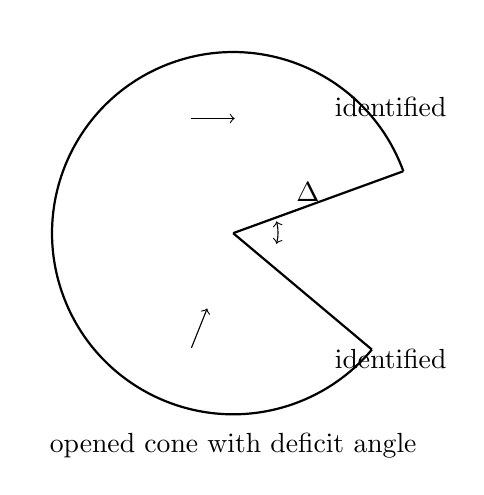
\begin{tikzpicture}[scale=1.0]
\draw[thick] (0,0) -- (20:2.3);
\draw[thick] (0,0) -- (320:2.3);
\draw[thick] (20:2.3) arc (20:320:2.3);
\draw[->] (110:1.55) -- ++(0.55,0);
\draw[->] (250:1.55) -- ++(0.20,0.50);
\draw[<->] (0.55,0.15) arc (15:-15:0.55);
\node at (0.95,0.52) {$\Delta$};
\node at (2.0,1.6) {identified};
\node at (2.0,-1.6) {identified};
\node at (0,-2.7) {opened cone with deficit angle};
\end{tikzpicture}
\caption{Schematic reconstruction of the conical-deficit argument used in the lecture. When the two radial edges are identified, a vector transported around the tip fails to return with the same direction.}
\end{figure}

Now carry a vector around the tip, keeping it parallel to itself as best the geometry allows. In the language already developed, we transport it so that its covariant derivative along the path is zero. When the vector returns, it is rotated. That rotation is the geometric effect of curvature.

This is the first picture of what curvature does. But the lecture then gives the algebraic version, which is more useful. Take a vector field and differentiate it in one direction, then in a second direction. Compare that with doing the same two differentiations in the opposite order. In flat space the order does not matter. In curved space it does.

\begin{figure}[h]
\centering
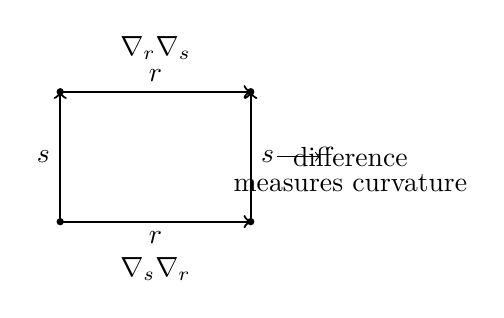
\begin{tikzpicture}[scale=1.1]
\fill (0,0) circle (1.2pt);
\fill (2.2,0) circle (1.2pt);
\fill (0,1.5) circle (1.2pt);
\fill (2.2,1.5) circle (1.2pt);
\draw[->,thick] (0,0) -- (2.2,0) node[midway,below] {$r$};
\draw[->,thick] (2.2,0) -- (2.2,1.5) node[midway,right] {$s$};
\draw[->,thick] (0,0) -- (0,1.5) node[midway,left] {$s$};
\draw[->,thick] (0,1.5) -- (2.2,1.5) node[midway,above] {$r$};
\node at (1.1,-0.55) {$\nabla_s\nabla_r$};
\node at (1.1,2.0) {$\nabla_r\nabla_s$};
\node at (3.35,0.75) {difference};
\node at (3.35,0.45) {measures curvature};
\draw[->] (2.5,0.75) -- (3.0,0.75);
\end{tikzpicture}
\caption{The two orders of covariant differentiation correspond to the two ways of moving around a small loop. Their difference is the local curvature probe.}
\end{figure}

The differential statement is
\begin{equation}
(\nabla_s\nabla_r-\nabla_r\nabla_s)V_n
=
R^{t}{}_{nrs}V_t.
\end{equation}
This defines the Riemann curvature tensor \(R^{t}{}_{nrs}\). In canonical Levi-Civita form,
\begin{equation}
R^{t}{}_{nrs}
=
\partial_r\Gamma^{t}{}_{sn}
-
\partial_s\Gamma^{t}{}_{rn}
+
\Gamma^{p}{}_{sn}\Gamma^{t}{}_{rp}
-
\Gamma^{p}{}_{rn}\Gamma^{t}{}_{sp}.
\end{equation}

Here the lecture wants us to notice one thing above all. The Christoffel symbols contain first derivatives of the metric. Therefore the first two terms in \(R^{t}{}_{nrs}\) contain second derivatives of the metric, and the last two contain quadratic combinations of first derivatives. This is exactly right. First derivatives of the metric can be made to vanish at a point by Gaussian normal coordinates. Second derivatives cannot, in general. So the curvature tensor feels precisely the part of the metric variation that cannot be transformed away.

If every component of \(R^{t}{}_{nrs}\) vanishes everywhere, the space is flat. That is the promised diagnostic. It is still an infinite problem point by point, but it is a vastly better infinite problem than searching over all coordinate systems at every point. If the metric is given analytically, one differentiates, computes \(R\), and checks whether the analytic result vanishes.

\subsection{Question \& Answer}

\paragraph{Question.} What distinguishes a real gravitational field from acceleration?

\paragraph{Answer.} Tidal forces. An accelerated frame can imitate many features of gravity, but it does not produce tidal distortion. Real gravity, produced by real matter, varies from place to place and creates relative stretching and squeezing. That local invariant content is exactly what the curvature tensor measures.

The lecture closes by making this identification explicit. Curvature is not merely a mathematical inconvenience. It is the geometric form of tidal force. Small objects may not feel it much, because over a sufficiently small body the field hardly changes. Large objects do feel it, because different parts of the body sample different local geometry. That is why one can fall freely in a small elevator and feel almost nothing, yet a sufficiently extended body in the same gravitational environment will be stretched and compressed.

So the progression is complete. We began by asking how to distinguish real geometry from funny coordinates. We found that local flatness hides all first-order information, that naive differentiation is not tensorial, that covariant differentiation repairs the defect, and that the failure of covariant derivatives to commute finally exposes the curvature tensor. In physics language, that same tensor is what we call tidal force.

\section{Summary}

This lecture builds the diagnostic machinery that gravity needs. The metric gives lengths, raises and lowers indices, and locally can always be made to look Euclidean through first order. That local simplification, however, destroys the naive derivative as a tensorial notion and forces us to introduce the covariant derivative together with the Christoffel symbols. The Christoffel symbols themselves are coordinate data, not curvature. Curvature only appears when we compare two orders of covariant differentiation or, geometrically, when we transport a vector around a small loop and fail to get back what we started with.

The central payoff is the Riemann tensor. It is the object that vanishes in flat space and becomes nonzero when geometry carries real invariant content. In the next lecture the same mathematical structure will be reinterpreted directly as gravity, and the discussion will move from Riemannian geometry to Einstein geometry and then to the Schwarzschild example.